\documentclass[11pt]{article}

\usepackage[T1]{fontenc}
\usepackage{geometry}
\usepackage{amsmath, amssymb, amsthm}
\usepackage[scr]{rsfso}
\usepackage[%
    hidealllines=true,%
    innerbottommargin=15,%
    nobreak=true,%
]{mdframed}
\usepackage{xcolor}
\usepackage{graphicx}
\usepackage{fancyhdr}
\usepackage{hyperref}

\geometry{a4paper, margin=1in, headheight=14pt}

\pagestyle{fancy}
\fancyhf{}
\renewcommand\headrulewidth{0.4pt}
\fancyhead[L]{\scshape MA3103}
\fancyhead[R]{\scshape \leftmark}
\rfoot{\footnotesize\it Updated on \today}
\cfoot{\thepage}

\newcommand{\C}{\mathbb{C}}
\newcommand{\R}{\mathbb{R}}
\newcommand{\Q}{\mathbb{Q}}
\newcommand{\Z}{\mathbb{Z}}
\newcommand{\N}{\mathbb{N}}

\newmdtheoremenv[%
    backgroundcolor=blue!10!white,%
]{theorem}{Theorem}[section]
\newmdtheoremenv[%
    backgroundcolor=violet!10!white,%
]{corollary}{Corollary}[theorem]
\newmdtheoremenv[%
    backgroundcolor=teal!10!white,%
]{lemma}[theorem]{Lemma}

\theoremstyle{definition}
\newmdtheoremenv[%
    backgroundcolor=green!10!white,%
]{definition}{Definition}[section]
\newmdtheoremenv[%
    backgroundcolor=red!10!white,%
]{exercise}{Exercise}[section]

\theoremstyle{remark}
\newtheorem*{remark}{Remark}
\newtheorem*{example}{Example}
\newtheorem*{solution}{Solution}

\surroundwithmdframed[%
    linecolor=black!20!white,%
    hidealllines=false,%
    innertopmargin=5,%
    innerbottommargin=10,%
    skipabove=0,%
    skipbelow=0,%
]{example}

\numberwithin{equation}{section}

\title{
    \Large\textsc{MA3103} \\
    \Huge \textbf{Introduction to Graph Theory and Combinatorics} \\
    \vspace{5pt}
    \Large{Autumn 2021}
}
\author{
    \large Satvik Saha
    \\\textsc{\small 19MS154}
}
\date{\normalsize
    \textit{Indian Institute of Science Education and Research, Kolkata, \\
    Mohanpur, West Bengal, 741246, India.} \\
}

\begin{document}
    \maketitle

    \tableofcontents

    \section{Introduction}
    
    \subsection{The Seven Bridges of K\"onigsberg}
    
    The diagram below depicts a region in the city of K\"onigsberg, Prussia. There
    are two islands, connected with the mainland and to each other via seven bridges.
    The Seven Bridges Problem is posed as follows: is it possible to walk through the
    entire city, visiting each one of the four landmasses by crossing each of the
    bridges exactly once?

    \begin{center}
        \includegraphics[width=0.6\textwidth]{7_bridges.png}
    \end{center}

    Leonhard Euler showed that this is impossible; no such walk exists. The
    techniques he developed in doing so laid the foundations of \textit{graph
    theory}.

    The first thing to note is that the exact shape of the walk/trail is immaterial;
    all that matters is the sequence of landmasses visited and bridges crossed. Thus,
    each landmass can be compacted to a single point or \textit{vertex}, and each
    bridge a line or \textit{edge} connecting two such points. The resulting figure
    is a graph. Note that the orientations or placements of the points and lines are
    irrelevant, as long as the connections are undisturbed.

    \begin{center}
        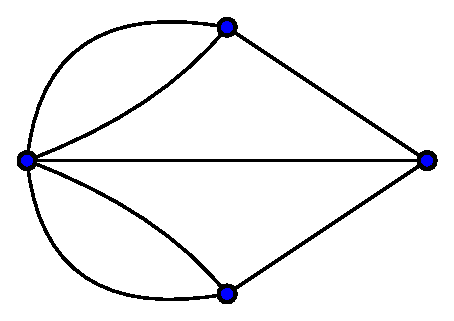
\includegraphics[width=0.5\textwidth]{7_bridges_graph.eps}
    \end{center}

    Now, examine a landmass which is on the trail but is neither our starting point,
    nor our ending point. In order to reach this landmass, we must enter via a bridge; but
    we cannot stay in the landmass, so we must leave via another a bridge. Thus, for
    each time we pass through this landmass, we can cross off two bridges joined to
    it. Once we are done, no bridge may remain unused; this means that we must have
    started with an even number of bridges joined to this landmass.

    However, all four vertices in our graph connect to an odd number of edges. Since
    we require at least two vertices to act as intermediate points on our path, the
    desired walk is impossible.

    \subsection{Basic definitions}
    \begin{definition}
        A graph $G(V, E)$ is an ordered pair of the set of vertices $V$ and the set
        of edges $E$.
    \end{definition}
    \begin{definition}
        A simple graph is undirected, unweighted, and contains no self-loops or
        multiple edges joining vertices.
    \end{definition}
    \begin{definition}
        For a simple undirected graph, the set of edges $E$ consists of two-element
        subsets of the set of vertices $V$.
        \begin{remark}
            For a directed, unweighted graph, the set of edges $E$ consists of ordered
            pairs of elements from the set of vertices $V$.
        \end{remark}
    \end{definition}
    \begin{definition}
        A vertex is incident to an edge if that edge joins that vertex.
    \end{definition}
    \begin{definition}
        Two vertices are adjacent if there exists an edge connecting them.
        Two edges are adjacent if they connect to a common vertex.
    \end{definition}
    \begin{definition}
        The neighbours of a vertex consist of all vertices adjacent to it.
        The neighbours of an edge consist of all edges adjacent to it.

        The number of neighbours of a vertex is called the degree of that vertex.
    \end{definition}

    \begin{definition}
        A complete graph is such that every pair of vertices is connected by an
        edge. The complete (simple) graph of $n$ vertices is denoted by $K_n$.
    \end{definition}

    \subsection{Some principles}
    
    \begin{lemma}[Pigeonhole Principle]
        If $n + 1$ objects are placed in $n$ boxes, then we can fin a box containing
        at least $2$ objects.
    \end{lemma}
    \begin{proof}
        If every box contains at most $1$ objects, then the total number of objects
        falls short.
    \end{proof}

    \begin{theorem}
        There are no simple graphs where the degrees of all vertices are distinct.
    \end{theorem}
    \begin{proof}
        Let $G(V, E)$ be a simple graph with $n$ vertices. The degrees of each of
        these vertices must be an integer among $0, 1, \dots, n - 1$. We now consider
        two cases. \\

        \textbf{Case I}: There is a vertex of degree $0$. Thus, this vertex is
        adjacent to no other vertex, which means that no vertex can have the full
        degree $n - 1$. This means that the remaining vertices have degrees among $1,
        2, \dots, n - 2$, i.e.\ $n - 2$ choices of degree for $n - 1$ vertices.

        \textbf{Case II}: There is no vertex of degree $0$. Thus, the vertices have
        degrees among $1, 2, \dots, n - 1$, i.e.\ $n - 1$ choices of degree for $n$
        vertices. \\

        In either case, the Pigeonhole Principle forces at least two vertices to
        share the same degree.
    \end{proof}

    \begin{lemma}[Strong Pigeonhole Principle]
        Let $q_1, q_2, \dots, q_n$ be positive integers. If \[
            N = q_1 + \dots + q_n - n + 1
        \] objects are placed in $n$ boxes, then we can find a box $i$ containing at
        least $q_i$ objects.
    \end{lemma}
    \begin{proof}
        If every box $i$ contains at most $q_i - 1$ objects, then the total number of
        objects falls short. \[
            N \leq (q_1 - 1) + \dots + (q_n - 1) = q_1 + \dots + q_n - n = N - 1 \qedhere
        \] 
    \end{proof}

    \begin{theorem}
        The sum of the degrees of all vertices in a simple graph is twice the number
        of its edges. 
    \end{theorem}
    \begin{proof}
        Let $G((V, E)$ be a simple graph. 
        Define the incidence function $I\colon E \times V \to \{0, 1\}$, such that
        $I(e, v) = 1$ if $e$ and $v$ are incident, $0$ otherwise. We perform the
        double counting, \[
            \sum_{v\in V}\sum_{e \in E} I(e, v) = \sum_{e \in E}\sum_{v \in V} I(e,
            v).
        \] Now, the number of edges incident to a vertex is simply its degree, so
        $\sum_{e \in E} I(e, v) = d(v)$. Also, every edge is incident to exactly two
        vertices, so $\sum_{v \in V} I(e, v) = 2$. Thus, we have \[
            \sum_{v \in V} d(v) = 2 |E|. \qedhere
        \] 
    \end{proof}

    \begin{lemma}[Inclusion-Exclusion Principle]
        For finite sets $A_1, A_2, \dots, A_n$, the number of elements in their union
        is given by \[
            \sum_{i=1}^n |A_i| - \sum_{1 \leq i < j \leq n} |A_i\cap A_j| +
            \sum_{1 \leq i < j < k \leq n} |A_i \cap A_j\cap A_k| - \dots + 
            (-1)^{n-1} \left|A_1\cap\cdots\cap A_n\right|.
        \] 
    \end{lemma}

    \begin{theorem}
        There are $2^{\binom{n}{2}}$ simple graphs with $n$ vertices.
    \end{theorem}
    \begin{exercise}
        How many simple graphs are there with $n$ vertices and $m$ edges?
    \end{exercise}
    \begin{theorem}
        Let $n, k \in \N$ such that $n > 3$ and $n / 2 < k < n$. Let there be $n$
        points on a plane such that no three points are collinear. If every point is
        connected to at least $k$ other points by segments, then there must be at
        least three segments forming a triangle.
    \end{theorem}
    \begin{proof}
        Consider a graph $G(V, E)$ with $n$ vertices, such that every vertex has
        degree at least $k$. Pick an edge, say $\{x, y\}$, and let $A$ be the
        neighbours of $x$ apart from $y$, $B$ be the neighbours of $y$ apart from
        $x$. Note that $A$, $B$ have at least $k - 1$ elements each. Suppose that $A
        \cap B = \emptyset$, i.e.\ the edge $\{x, y\}$ doe not form a triangle. Thus,
        \[
            |A\cup B| = |A| + |B| - |A \cap B| \geq 2(k - 1).
        \] However, $|A\cup B| \leq n - 2$, hence $n \geq 2k$, or $k \leq n / 2$.
        This is a contradiction.
    \end{proof}
    \begin{remark}
        We have shown that \emph{every} segment is part of a triangle. The number of
        segments here is \[
            |E| \geq n k > \frac{n^2}{4}.
        \] 
    \end{remark}
    \begin{exercise}
        Is the condition $|E| > n^2 / 4$ sufficient to ensure the existence of a triangle?
    \end{exercise}

    \begin{lemma}[Cauchy-Schwarz]
        Let $a_1, \dots, a_n$ and $b_1, \dots, b_n$ be positive reals. Then, \[
            (a_1^2 + \dots + a_n^2) (b_1^2 + \dots + b_n^2) \geq (a_1b_1 + \dots +
            a_nb_n)^2.
        \] Equality holds if and only if every $a_i = \lambda b_i$ for some fixed
        real $\lambda$.
    \end{lemma}

    \begin{theorem}[Mantel]
        In a simple graph with $n$ vertices, the condition $|E| > n^2 / 4$ is
        sufficient to ensure the existence of a triangle.
    \end{theorem}
    \begin{proof}
        Let $G$ be a simple graph with $n$ vertices which is triangle-free. Thus, for
        any edge $\{x, y\} \in E$, the neighbour sets $A$ and $B$ of $x$ and $y$
        intersect at no vertex. Thus, we can write \[
            d(x) + d(y) = |A \cup B| \leq n.
        \] Sum this over all possible edges. On the right, we have $n|E|$. On the
        left, we have the sum \[
            \sum_{x \in V} d(x)^2 \geq \frac{1}{n} \left(\sum_{x \in V} d(x)\right)^2
            \geq \frac{1}{n} \cdot 4|E|^2
        \] This gives \[
            \frac{4|E|^2}{n} \leq n |E|, \qquad |E| \leq \frac{n^2}{4}. \qedhere
        \] 
    \end{proof}
    \begin{example}
        Consider a circle, with 21 points on its circumference. It follows that among
        the angles subtended by these points at the center, at most 110 are greater
        than $2\pi / 3$. \\

        Note that there are $\binom{21}{2} = 210$ angles. Furthermore, given any 3
        points on the circle (forming a triangle), all three angles subtended by them
        cannot be greater than $2\pi / 3$. Construct a graph with these $n = 21$
        points as vertices, such that two vertices are connected by an edge if and
        only if the angle subtended by them is greater than $2\pi / 3$.  Now, note
        that $n^2 / 4 = 110.25$, thus if there are more than $110$ edges, there must
        exist a triangle of vertices in which all three angles are greater than $2\pi
        / 3$ -- a contradiction!
    \end{example}

    \subsection{Bipartite graphs}
    \begin{definition}
        A graph $G(V, E)$ is called bipartite if the vertex set $V$ can be
        partitioned into 2 parts $V_1$, $V_2$ such that every edge in $E$ joins a
        vertex of $V_1$ to a vertex of $V_2$. In other words, there exists a 2-
        colouring of the vertices such that no edge connects two vertices of the same
        colour.

        \begin{remark}
            The sum of the degree of the vertices in one part is exactly equal to
            the number of edges, which in turn is equal to the sum of the degrees of
            the vertices in the other part.
        \end{remark}
    \end{definition}

    \begin{definition}
        A complete bipartite graph is such that each vertex in one part is connected
        to every vertex in the other part. Such a graph is denoted by $K_{m,n}$,
        where the parts have $m$ and $n$ vertices respectively.

        \begin{remark}
            The total number of edges must be the product of the numbers of vertices
            in each part.
        \end{remark}
    \end{definition}

    \begin{definition}
        A set of vertices (or edges) in a graph is called independent if no two
        elements in that set are adjacent.
    \end{definition}

    \begin{lemma}
        A bipartite graph is triangle free.
    \end{lemma}

    \begin{corollary}
        If we choose even $n$, we can achieve a triangle free graph with $n^2 / 4$
        edges, namely $K_{n / 2, n / 2}$
    \end{corollary}

\end{document}
